%
% div.tex -- Konvergenz eines Iterationsverfahrens
%
% (c) 2019 Prof Dr Andreas Müller, Hochschule Rapperswil
%
\documentclass[tikz]{standalone}
\usepackage{amsmath}
\usepackage{times}
\usepackage{txfonts}
\usepackage{pgfplots}
\usepackage{csvsimple}
\usetikzlibrary{arrows,intersections,math}
\begin{document}
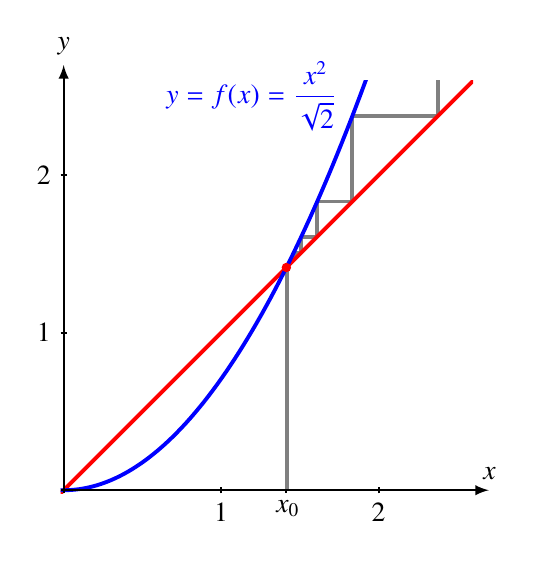
\begin{tikzpicture}[>=latex,scale=2]

\draw[line width=0.3pt] (1.4142,1.4142)--(1.4142,0);
\draw[line width=0.7pt] (1.4142,0.02)--(1.4142,-0.02);
\node[color=white] at (1.4142,0.02) [below] {$\sqrt{2}$};

\foreach \i in {1,...,2}{
	\draw[line width=0.7pt] ({\i},-0.02)--({\i},0.02);
	\node at ({\i},-0.02) [below] {$\i$};
	\draw[line width=0.7pt] (-0.02,{\i})--(0.02,{\i});
	\node at (-0.02,{\i}) [left] {$\i$};
}

\xdef\xold{1.42}
\xdef\yold{0}
\xdef\x{\xold}
\pgfmathparse{\x*\x/1.4142}
\xdef\y{\pgfmathresult}

\node at ({\xold},{\yold}) [below] {$x_0$};

\begin{scope}
\clip (-0.02,-0.02) rectangle (2.6,2.6);

\draw[color=gray,line width=1.4pt] ({\xold},{\yold})--({\x},{\y});

\xdef\xold{\x}
\xdef\yold{\y}
\xdef\x{\y}

\draw[color=gray,line width=1.4pt] ({\xold},{\yold})--({\x},{\y});


\foreach \i in {0,...,6}{

\ifnum \i > 3
	\ifnum \i < 2
		\node at ({\xold},{\yold}) [below] {$x_\i$};
	\fi
\fi

\xdef\xold{\x}
\xdef\yold{\y}
\xdef\x{\xold}
\pgfmathparse{\x*\x/1.4142}
\xdef\y{\pgfmathresult}

\draw[color=gray,line width=1.4pt] ({\xold},{\yold})--({\x},{\y});

\xdef\xold{\x}
\xdef\yold{\y}
\xdef\x{\y}

\draw[color=gray,line width=1.4pt] ({\xold},{\yold})--({\x},{\y});
}


\draw[line width=1.4pt,color=red] (-1,-1)--(3,3);

\draw[color=blue,line width=1.4pt] plot[domain=-0.1:2.7,samples=100]
	({\x},{\x*\x/1.4142});

\end{scope}

\fill[color=red] (1.4142,1.4142) circle[radius=0.03];

\draw[->,line width=0.7pt] (-0.02,0)--(2.7,0) coordinate[label={$x$}];
\draw[->,line width=0.7pt] (0,-0.02)--(0,2.7) coordinate[label={$y$}];

\node[color=blue] at (1.8,2.5) [left] {$y=f(x) =\displaystyle \frac{x^2}{\sqrt{2}}$};

\end{tikzpicture}
\end{document}

